\documentclass[12pt]{article}
\usepackage[margin=1in]{geometry}
\usepackage{amsmath}
\usepackage{amsthm}
\usepackage{float}
\usepackage{graphicx}
\usepackage{natbib}
\usepackage{enumitem}
\usepackage{booktabs}
\usepackage{hyperref}
\usepackage[utf8]{inputenc}
\usepackage{lipsum}
\usepackage[english]{babel}
\usepackage[autostyle, english = american]{csquotes}
\MakeOuterQuote{"}
\title{Call Center Regression Data Analysis}

\author{Michael  Marcaccio}

\date{November 14 2022}

\begin{document}

\maketitle

\begin{abstract}
 With over 15 million people employed, a compound annual growth rate (CAGR) of 5.6 percent between 2020 and 2027, and 28,000
 in the United States alone, call centers play a pivotal role in a businesses success.In this paper, call center volume was forecasted and
 models were created to predict the number of agents needed to meet critical attributes such as waittime, calltime, and holdtime. 
 Forecasting gives businesses the ability to make informed business decision and develop data-driven strategies. In the literature it is very
 common to see call center volume being predicted using different techniques, but there is very limited studies on attempting to correlate
 the number of agents needed. Through Regression techniques, there are 8 models proposed to model the number of agents needed based on waittime,
 calltime, goaltime, and the amount of calls handled.
\end{abstract}

\section*{Introduction}
With over 15 million people employed, a compound annual growth rate (CAGR) of 5.6 percent between 2020 and 2027, and 28,000
in the United States alone, call centers play a pivotal role in a businesses success. Call Centers are a key part of customer service,
that will save a company time, money, and unneccessary stress. In the banking industry, calls can range from inquires, transfers, 
payments, reporting, to processing. This means members can be calling about their account balance, credit card bills, loan applications, 
or unauthorized transactions. It is crucial that a bank is prepared for spikes in calls and have agents knowledgeable in all aspects of the bank.




    
\section*{Data Description}



\section*{Methods}
Test stuffg
\begin{figure}[H]
    \centering
    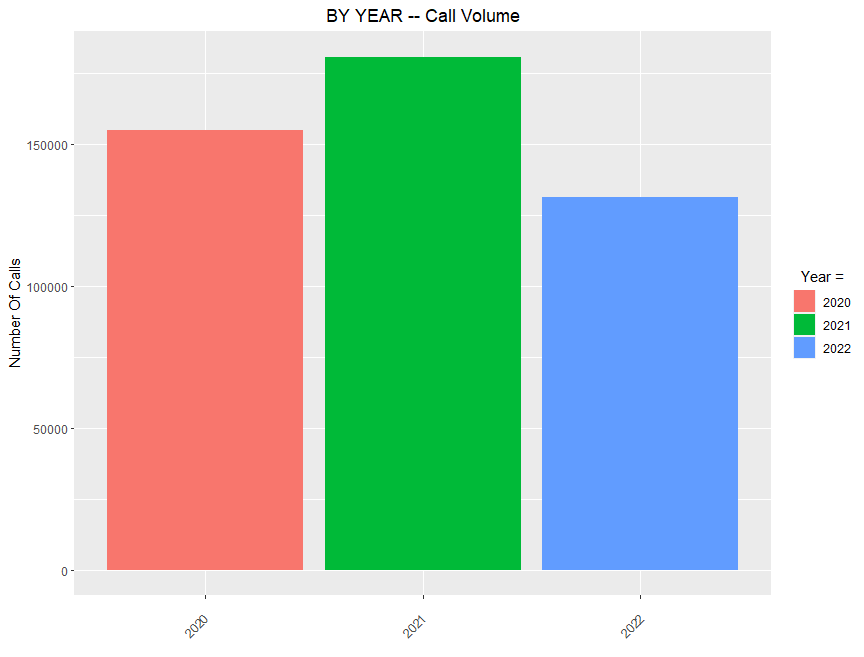
\includegraphics[width=200pt,height=200pt]{By Year.png}
    \caption{This is my first figure.}
    \label{fig:Year}
  \end{figure}

\section*{Results}
\citep{avramidis2005modeling}
\citep{evensen1999effective}
\citep{ibrahim2016modeling}


\section*{Discussion}


\bibliographystyle{chicago}
\bibliography{Citations.bib}
\end{document}